\section{Video Input}
After some consideration it was decided that the \textit{Raspberry Pi Camera Board}\footnote{\url{https://www.raspberrypi.org/products/camera-module/}} (PiCamera) would be used as the camera module for the system.
The circumstances leading to this choice are discussed in section \ref{sec:camera_discussion}.
In addition to the camera, a backup scheme with video from the SD card controlled by the MCU was also planned.
Lastly, a second HDMI port was also added to the board, opening the possibility of HDMI input.

\subsection{Raspberry Pi Camera}
After some consideration it was decided that the \textit{Raspberry Pi Camera Board}\footnote{\url{https://www.raspberrypi.org/products/camera-module/}} (PiCamera) would be used as the camera module for the system.
The circumstances leading to this choice are discussed in Section \ref{sec:camera_discussion}.

\begin{figure}[h]
    \centering
    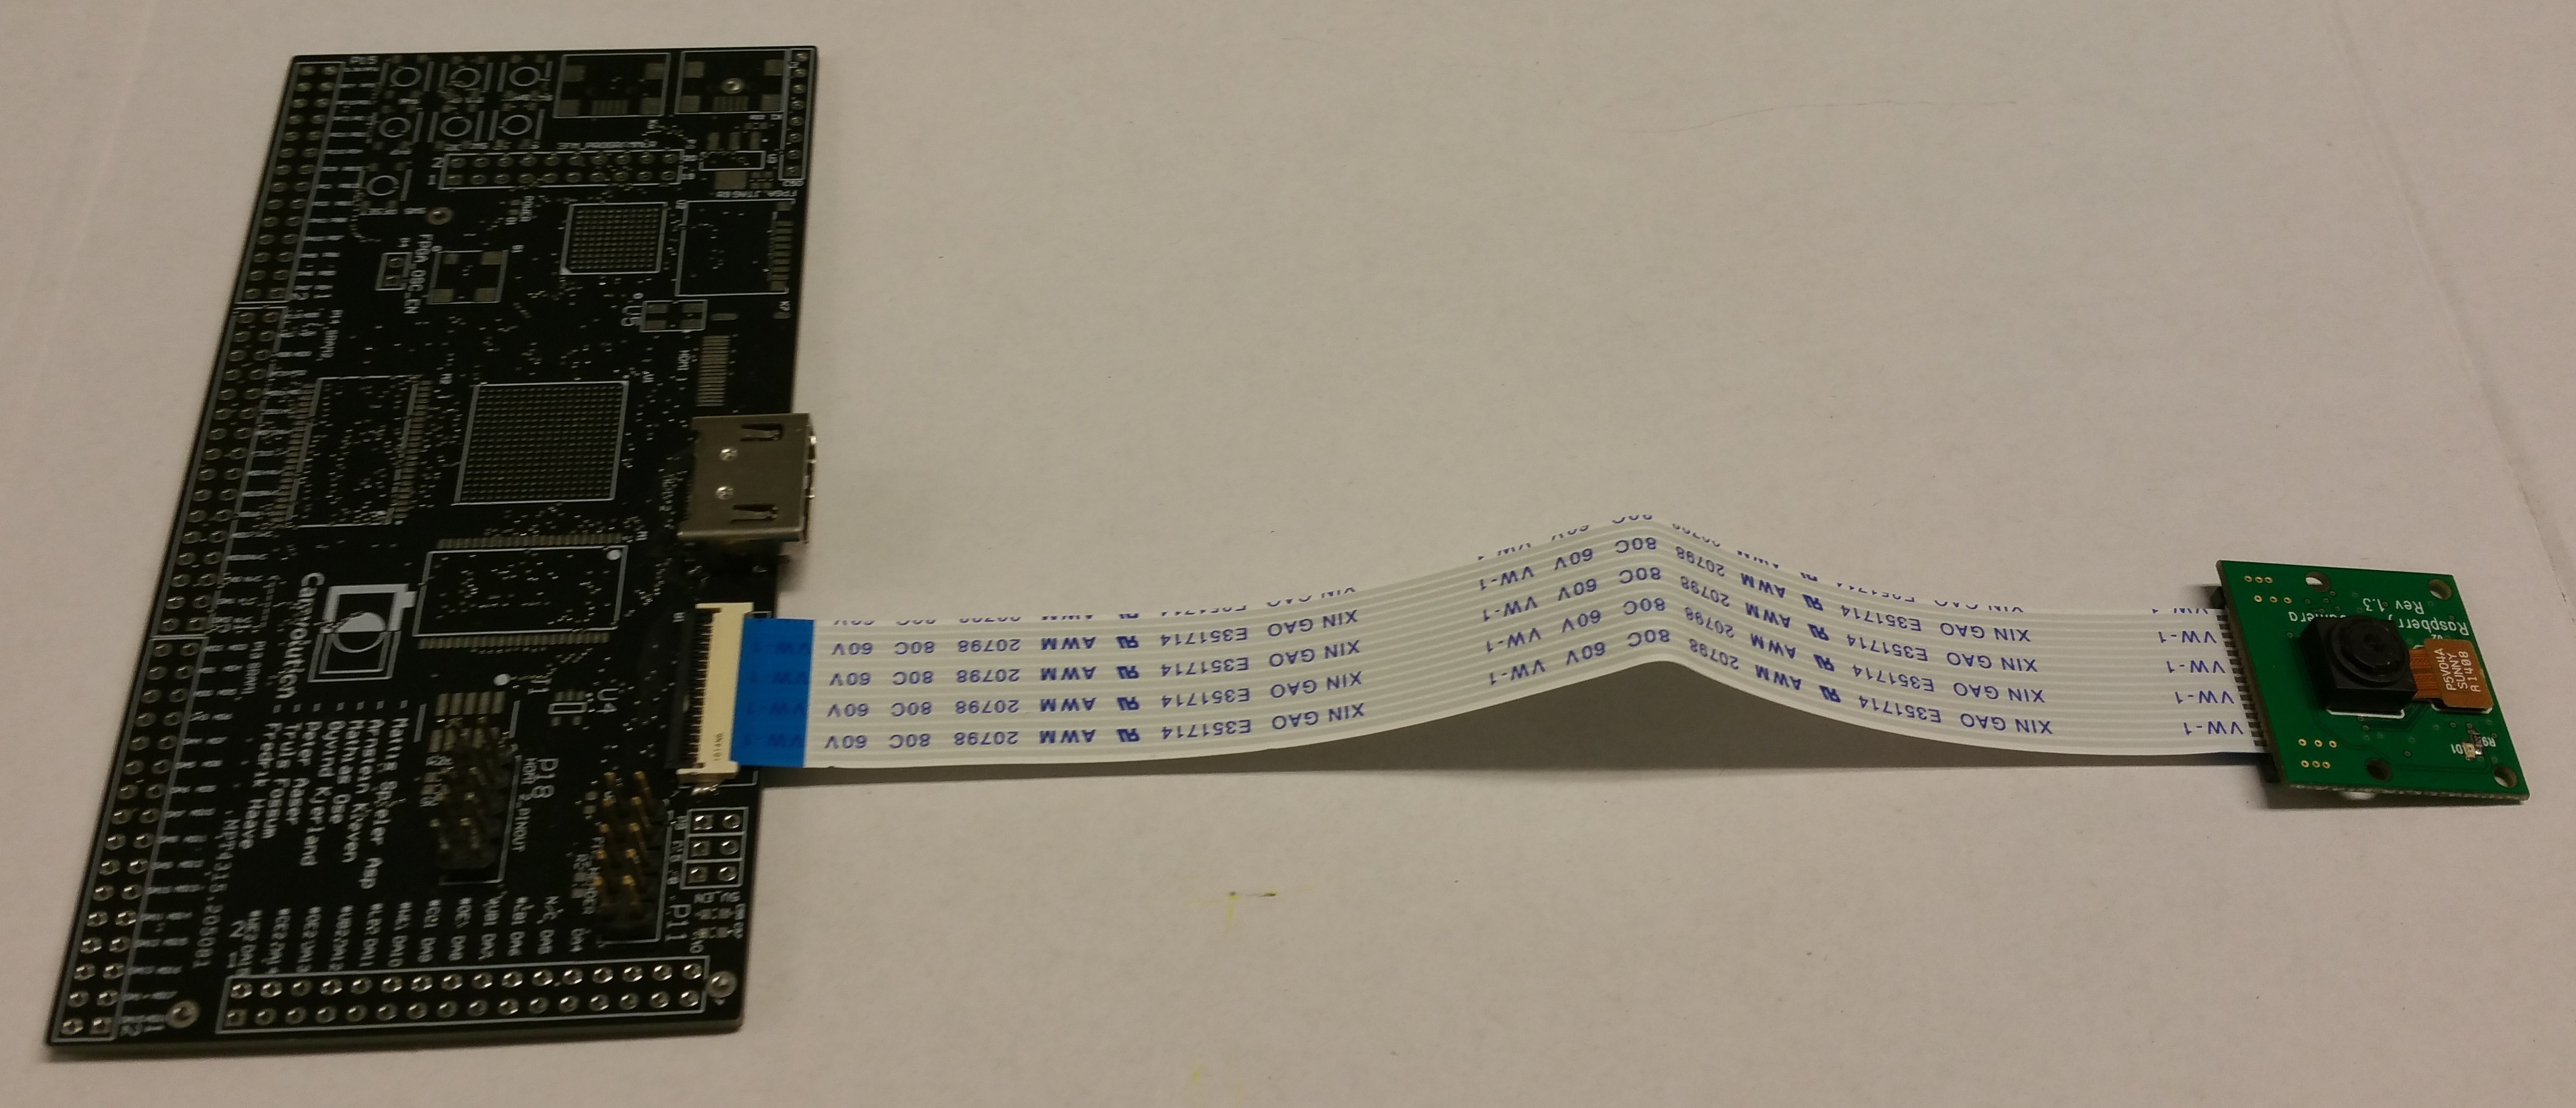
\includegraphics[width=0.75\textwidth]{img/picamera}
    \caption{Raspberry Pi Camera connected to Camvolution board}
\end{figure}

The \textit{Raspberry Pi Foundation} has designed this peripheral for use with the \textit{Raspberry Pi} computer.
The PiCamera can take still shots as well as record continuous video.
The module consists of a camera sensor on a board with a controller unit which connects to the Pi (or another master device) via a 16-pin ribbon cable.
Communication over this cable is defined by the proprietary \textit{MIPI Camera Serial Interface} (CSI) specification.

The master device controls the camera module by sending instructions over an I2C bus on the ribbon cable,
and the camera module responds with picture data over two clocked differential busses.\cite{picam-pinout}
Parameters that may be controlled include video encoding, resolution in two dimensions and framerate.


\subsection{SD Card Video}
One possible source of video is a file stored on the SD card connected to the board.
The MCU is able to open files and pass the data from it to the processor over EBI.
For simplicity of development the MCU should not need to handle encoded video. Instead, the video files should contain raw pixel data so that it can easily be streamed to the processor.


\subsection{Options for Video Path}
There were several options for how to move the video stream to the processor,
as illustrated by Figure \ref{fig:VideoPath}.

\begin{figure}
    \centering
    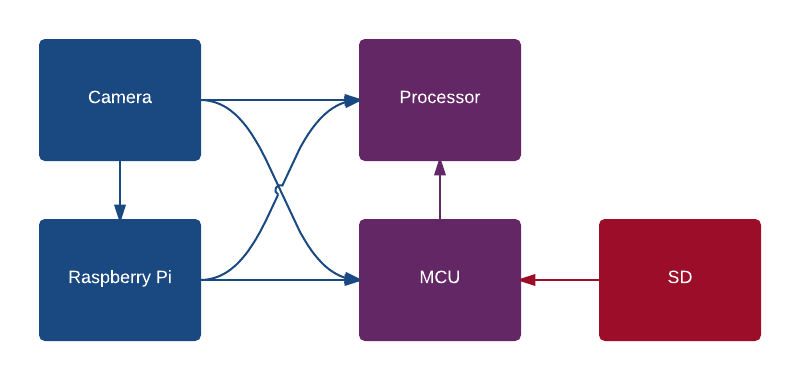
\includegraphics[width=\linewidth]{img/VideoPath}
    \caption{Paths an input video stream could take to reach the processor.}
    \label{fig:VideoPath}
\end{figure}

\subsubsection{MCU as Camera Master}
\begin{figure}
    \centering
    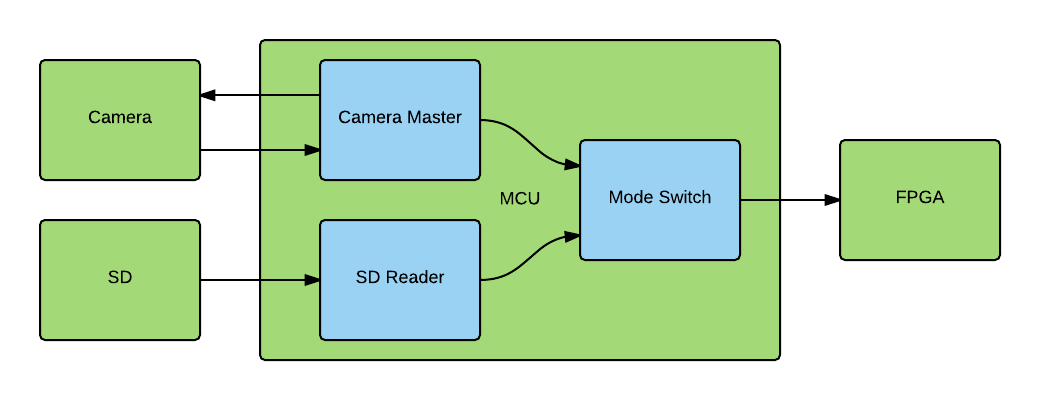
\includegraphics[width=\linewidth]{img/MCU_CameraMaster}
    \caption{MCU as input controller. Hardware components in green, software components in blue.}
    \label{fig:MCU_CameraMaster}
\end{figure}

The first possibility we explored was to have the MCU be the camera master.
It would send commands to the camera module and receive video input.
With this setup the MCU would have the responsibility of multiplexing input from camera or SD and the FPGA wouldn't have to know anything about the source of the video stream,
only that it comes via the MCU-FPGA connection.
Figure \ref{fig:MCU_CameraMaster} illustrates this.

\subsubsection{FPGA as Camera Master}
\begin{figure}
    \centering
    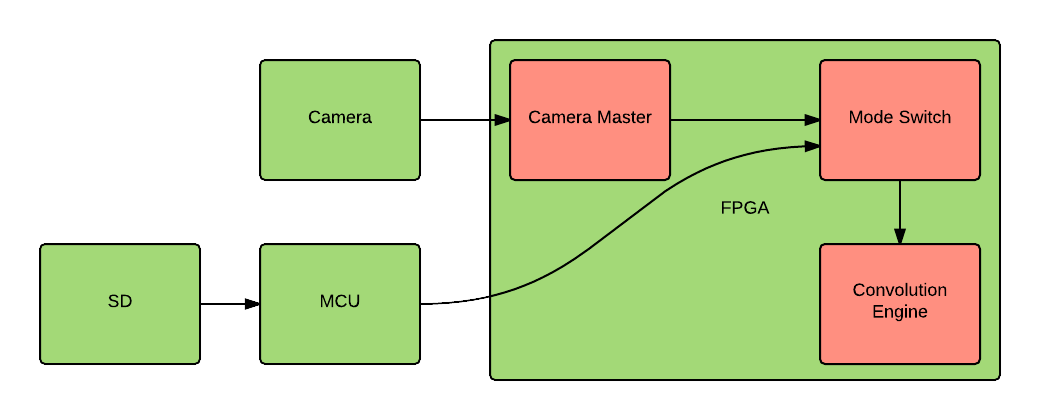
\includegraphics[width=\linewidth]{img/FPGA_CameraMaster}
    \caption{FPGA with input controller module. Hardware components in green, FPGA submodules in red.}
    \label{fig:FPGA_CameraMaster}
\end{figure}

Another option for system architecture would be to have the FPGA be camera master,
with another submodule in the FPGA switching between input from MCU and input from camera.

As we learned more about the PiCamera we came to the realization that the FPGA would be more appropriate to handle the differential bus data stream from the PiCamera.
We therefore pivoted and began working on a VHDL camera control module.
The first step for this would be to implement an I2C master module that would send control signals to the PiCamera.

It was at this point we started realizing how undocumented this control protocol was.
After searching online and inspecting the Raspbery Pi Python and C camera control libraries with no luck,
we tried attaching a logic analyser to listen in on the communication between the Raspberry Pi and the PiCamera when starting a recording.
With the logic analyzer we were able to save a recording of the I2C control communication,
which we tried to recreate with our VHDL camera control module.
While we were able to send the same data to the samme addresses,
we were not able to get any acknowledgements from the PiCamera on the control bus.
Efforts into figuring out why the PiCamera wouldn't respond were fruitless, so the idea was eventually abandoned.

\subsubsection{Using the Raspberry Pi}
We had little success in reverse-engineering the camera control protocol.
However, we did have the Raspberry Pi with the functioning camera control provided.

Our system could include a whole Raspberry Pi with a camera as the camera module.
Programming the Pi to start recording is very easy thanks to the provided software.
The challenge then would be to get the video stream out of the Raspberry Pi and into the processor.

\subsubsection{GPIO Pins}
The Raspberry Pi has GPIO pins that are controllable with software.
A script was written which could start a camera recording,
then output the pixel data it on a the GPIO pins as a parallel bus with one clock pin and 8 data pins.
This was very simple to implement, however it was also very slow.
With a Raspberry Pi 2 the best frequency achieved was ca. $600kHz$.

The Raspberry Pi also has hardware support for SPI over some of the GPIO pins.
Directing the video stream to this instead was more promising,
since the frequency of the clock in this mode was able to go up to a $32MHz$\footnote{\url{http://elinux.org/index.php?title=RPi\_SPI\#Speed\_2}},
which would be a massive improvement even if the transfer was serial instead of 8-bit parallel.
Unfortunately what was observed was that while the transfer of chunks of data was fast,
there were long delays between chunks.

\subsubsection{HDMI Output}
Seeing that all efforts into using the camera were either failing or at bet offering a tiny stream of data,
we decided to concentrate on the HDMI input of the Camvolution system.
The Raspberry Pi has HDMI out, so it would definently be possible to use the PiCamera with this setup.

